\documentclass{article}

\usepackage{listings}
\usepackage{color}
\usepackage{graphicx}
\usepackage{float}
\usepackage{amsmath}
\usepackage{subfig}
\usepackage{cite}
\usepackage{url}
\usepackage{amsmath}

\begin{document}

\title{Robotics - Localization and Prediction}

\author{Asan Agibetov (\texttt{plumdeq@gmail.com}), 
\and Jander Nascimento (\texttt{jbotnascimento@gmail.com}).
\and Universite Joseph Fourier}

\maketitle

\section{Localization of a mobile robot}

\subsection{Kalman filter}
%Explain how kalman works and why it can be applied in the case of the robot
Kalman filter is an implementation of Bayesian Filters, where the space state is represented by Gaussian distribution, which makes it easier for the implementation on the computer(we avoid calculating integrals, when we use ``original'' Bayesian filter). Of course there's a drawback of this method, when the system is non-linear like in the case of \textit{changemotion}\footnote{more on this in the following section}.
\subsubsection{Problem of localization using Kalman filter}
The process of localization of the mobile robot with Kalman filter is divided into 3 parts:

\begin{enumerate}
\item Prediction
\item Estimation
\item Determination
\end{enumerate}

During this lab session we're dealing with \textit{1D} motion of the robot, hence the state transition model $\mathbf{P_t}$ is a scalar and is equal to 1, as well as the control input model $\mathbf{B_t}$. Which greatly simplifies the implementation of the Kalman filter for this case. The actual implementation is straightforward and can be found in the source code.
\subsection{Testing data sets}
%run in couple data sets and explain what is going on
\subsubsection{Belief in our actions and sensor model}
\emph{Q} and \emph{R} are respectively related with the confidence in the action and in the observation. The influence of these coefficients maybe important depending on their value. The \textit{Q} parameter changes the value of predicting the \textit{covariance} of our \textit{expected} state i.e. the dispersion or the error range. As \textit{Q} grows so is our dispersion i.e. the noise of the \textit{action} is too big to be neglected, hence our \textit{precision} diminishes. The \textit{R} coefficient is inversely proportional to the Kalman gain \textit{K} i.e. as \textit{R} grows, \textit{K} gets lower. The Kalman gain is used to \textit{affine} our \textit{final} i.e. \textit{estimated} value based on the observation. If \textit{R} is too big i.e. the noise of the sensor model is too big to be neglected, the \textit{final} estimated value is less affected by the current observation. Otherwise our sensor model is almost perfect, thus its contribution to the final value is important.
\subsubsection{The limit of the Kalman filter}
As we mentioned earlier Kalman filter is a good implementation of Bayesian filters for \textit{linear} systems, or as we might call it in the \textit{perfect case} example - a \textit{unidirectional} motion. In the \textit{perfect case} example robot is only moving in one direction, and if we express \textit{displacement} of the robot as the function of time, the equation has only one root i.e. at any given time $t$, the position of robot $p_t$ is unique. Which is not the case in the \textit{changemotion} example, where robot moves several units to the right and then goes back towards its starting location. Now, if we plot the graph of robot's displacement we may behold that for any given position $p_t$ there might be several \textit{roots} i.e. times $t_i$ and $t_j$ s.t. $t_i \neq t_j$. And that's where Kalman filter fails to provide adequate results. Nevertheless it works very good for dynamic linear systems.

\section{Detection and Tracking of a Moving Object}

\subsection{Tracking}

The tracking means generate an inference about the motion of an object given a sequence of observations in time $t$. This tool has a variety of applications, like:

\begin{itemize}
\item Motion capture
\item Recognition of motion
\item Surveillance
\item Targeting
\end{itemize}

These are just a few examples. With observation over the environment is possible to extract theses informations but not all data collected are relevant. 

Tracking is thought to be an inference problem, due to the fact that we need to compile all measurements to estimate the object state. There exist basically two branches of models: linear and not linear dynamics.

Not linear is quite hard to work with and in general looks impossible to predict, but there are some trivial solutions for the  linear model, for instance applying Kalman filter.

The Kalman filter is applied in three steps: prediction, kalman gain and estimation(correction). The canonical equations can be seen below.

\begin{equation} \label{eq:prediction}
  Prediction\;:\; 
  \left\{ 
    \begin{array}{ c }
      \mu_{t+1} = \mu_t + A_t \\
      \Sigma_{t+1} = \Sigma_t + Q_t
    \end{array}
  \right.
\end{equation}

\begin{equation} \label{eq:kalman_gain}
  Kalman\;gain\;:\; K_t = \frac{\Sigma_{t+1}}{\Sigma_{t+1} + R_t}
\end{equation}

\begin{equation} \label{eq:estimation}
  Estimation\;:\; 
  \left\{ 
    \begin{array}{ c }
      \mu_{t+1} = \mu_{t+1} + K_t(O_t - \mu_{t+1}) \\
      \Sigma_{t+1} = (1 - K_t)\Sigma_{t+1}
    \end{array}
  \right.
\end{equation}

\subsection{Motion detection}

For motion detection, base on a collection of frames at each time-step, is possible to analyze the current frame based on the previous measurement using a \emph{background} image. Background image is a template in which will be contrasted with the obtained measurement so we can inference some characteristics in the environment, for instance: detect motion.

Background, also known as inter-image difference, consist in compare the frame to be analyzed with a background frame, according to the difference obtained form these two image we can infer motion in the analyzed frame. 

The background image can be created using the very first sensor measure. So to detect the motion we can state the Equation \ref{equa:detection}, but this is a naive approach and have a lot of drawbacks, for instance:
\begin{itemize}
\item background image can become obsolete in case of any change in the environment
\item the contrast between the background and current frame can give a very inaccurate information about the moving object, Figure \ref{fig:subtraction_result}.
\end{itemize}

\begin{figure}[H]
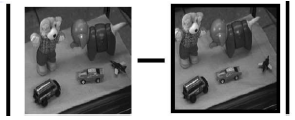
\includegraphics[scale=0.6]{image/subtraction.png}
\caption{Example: Given frame and background}
\label{fig:subtraction}
\end{figure}

\begin{figure}[H]
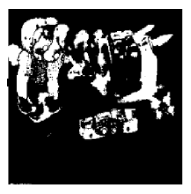
\includegraphics[scale=0.6]{image/subtraction_result.png}
\caption{Result of a subtraction \ref{fig:subtraction} for detecting the motion}
\label{fig:subtraction_result}
\end{figure}

\begin{equation}
motion(I_{frame})=\parallel I_{background}-I_{frame} \parallel
\label{equa:detection}
\end{equation}

if the result of the Equation \ref{equa:detection} is bigger than a \emph{threshold} is consider as a motion. This \emph{threshold} depends on the sensor confidence, and can varying from one model to other. 

\subsection{Kalman for DATMO}
%explain how the kalman is used for tracking
The Detection and Tracking of Moving Objects(DATMO) can be done using statistical methods. After performing and action and having an observation of the sensor it is possible to predict the next position by using Kalman Filter. 

Kalman Filter has some limitations:
\begin{itemize}
\item Environment to be analyzed must be discrete
\item The motion of the object must be a linear system
\end{itemize}

Considering the current model, is not possible to apply Kalman Filter since the model has 2 degrees of freedom, but is possible to simplify it considering that the robot is moving in only one axis (1D motion), this conversion is done by considering only the sensor that is pointing toward the motion of the robot.

\subsection{Training datasets}
%run in couple data sets and explain what is going on

\subsubsection{Motion detection}

The motion detection is performing checking up on the difference between two sensor measures, if this difference is bigger than a \emph{threshold} we consider as a motion. To display how accurate the algorithm is, a \textit{bounding box} is draw around the moving object.

But this approaches still give us some noisy in the sensor reading, the main problems faced with the datasets were:
\begin{itemize}
\item Motion detected where there was no motion
\item Larger bound-box than necessary
\end{itemize}

A proper detected bounding box can be seen in the Figure \ref{fig:boundbox01}.

\begin{figure}[H]
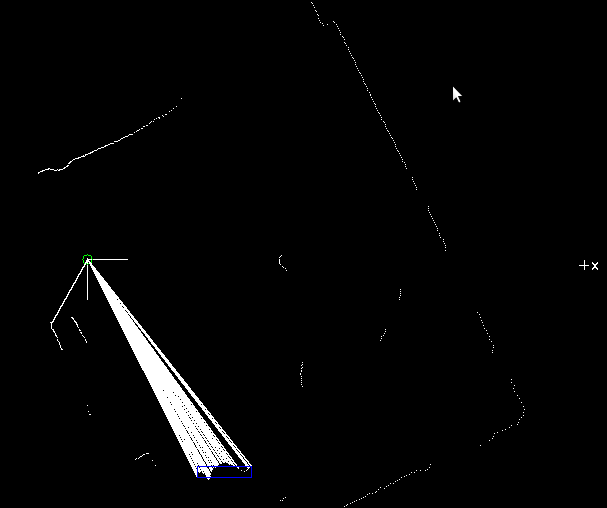
\includegraphics[scale=0.6]{image/boundbox01}
\caption{Perfectly detected boundbox}
\label{fig:boundbox01}
\end{figure}

To solve the problem of motion detection, we filtered the previous information using the technique called Laser Cluster, in which consist of group sensor measures, and if this measure is larger than a certain parameter we can consider it as a single object. 

Applying the Laser Cluster solved part of the problem, but in dataset \emph{Data2} for instance, there appear clustered lasers but that does not represent the actual moving object. The object was in the middle of the room and a sensor next to the object detected a false-motion in the back of the room.This situation can be seen in the Figure \ref{fig:boundbox02}

\begin{figure}[H]
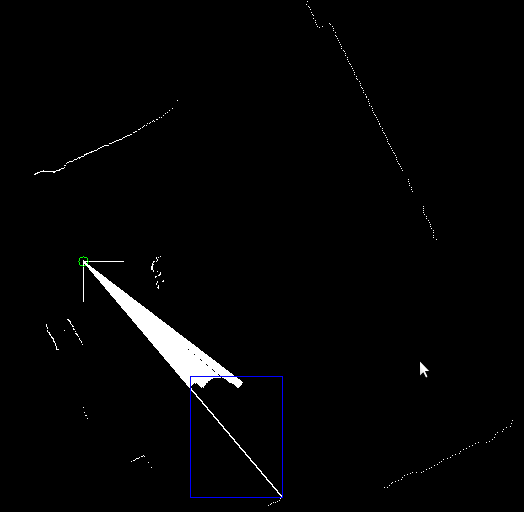
\includegraphics[scale=0.4]{image/boundbox02}
\caption{Boundbox with failure}
\label{fig:boundbox02}
\end{figure}


The solution what is called false cluster we can consider the distance between the elements of a cluster, if this distance is larger than a pre established value we can discard the measure at the longer distance. This implies most of the time for us, to know the size of the analyzed object, but this is not always possible. The result is Figure \ref{fig:boundbox03}

\begin{figure}[H]
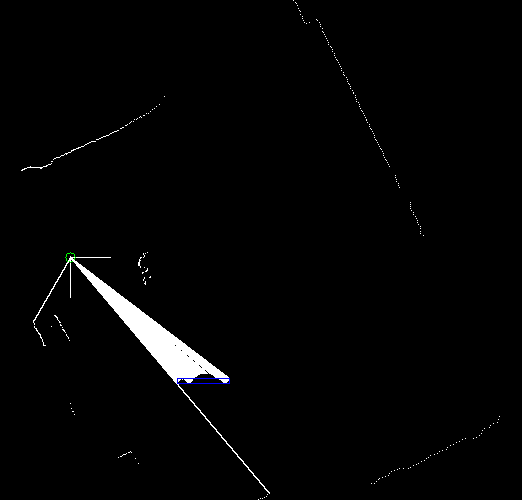
\includegraphics[scale=0.4]{image/boundbox03}
\caption{Correction using distance between the beans}
\label{fig:boundbox03}
\end{figure}


As we can see in the output below, the prediction error varies between 2 to 5. This informations was obtained from the DataSet1p, so it work quite well in this sample.

\begin{lstlisting}
mean(E) = 345 std(E) = 1.36633e-38
mean(P) = 350 std(P) = 4.00057e-34
observation = 344.8
mean(E) = 344 std(E) = 1.36633e-38
mean(P) = 350 std(P) = 4.00057e-34
observation = 345.3
mean(E) = 345 std(E) = 1.36633e-38
mean(P) = 352 std(P) = 4.00057e-34
observation = 344.4
mean(E) = 344 std(E) = 1.36633e-38
mean(P) = 349 std(P) = 4.00057e-34
observation = 345.2
mean(E) = 345 std(E) = 1.36633e-38
mean(P) = 350 std(P) = 4.00057e-34
observation = 345.4
mean(E) = 345 std(E) = 1.36633e-38
mean(P) = 349 std(P) = 4.00057e-34
observation = 344.9
mean(E) = 344 std(E) = 1.36633e-38
mean(P) = 349 std(P) = 4.00057e-34
observation = 344.9
mean(E) = 344 std(E) = 1.36633e-38
\end{lstlisting}

\section{Where to find the source}

The source code is available at \texttt{https://code.google.com/p/jfrobotics/source/browse/trunk/filter/Graphical/}.

To download the code run the following command:
\textit{svn export https://jfrobotics.googlecode.com/svn/trunk/filter/Graphical}

But is always possible to check the code straight from the web browser:
\texttt{https://code.google.com/p/jfrobotics/source/browse/}

\section{Appendix}

Between the two branches: Text and Graphical. Our team chose the \textbf{Graphical} for the visual feedback.

\end{document}


